\documentclass[fleqn,12pt]{article}
\usepackage[top=2cm, left=2cm,right=2cm,bottom=2cm]{geometry}
%\usepackage[fleqn]{amsmath}
\usepackage{amsmath}
\usepackage{url,multicol}
\usepackage{enumerate}
\usepackage{ifthen}
\newboolean{answers}
%\setboolean{answers}{true}  % set to true to include TODO statements
\setboolean{answers}{false}  % set to false to use input statements
\usepackage{amssymb}
\usepackage{tikz}
\newcommand{\<}{\ensuremath{\langle}}
\renewcommand{\>}{\ensuremath{\rangle}}
\newcommand{\ur}{\ensuremath{\underline{\mathrm{r}}}}
\newcommand{\uT}{\ensuremath{\underline{\mathrm{T}}}}
\newcommand{\uF}{\ensuremath{\underline{\mathrm{F}}}}
\newcommand{\uN}{\ensuremath{\underline{\mathrm{N}}}}
\newcommand{\ui}{\ensuremath{\underline{\mathrm{i}}}}
\newcommand{\uj}{\ensuremath{\underline{\mathrm{j}}}}
\newcommand{\ua}{\ensuremath{\underline{\mathrm{a}}}}
\newcommand{\ub}{\ensuremath{\underline{\mathrm{b}}}}
\newcommand{\un}{\ensuremath{\underline{\mathrm{n}}}}
\newcommand{\uv}{\ensuremath{\underline{\mathrm{v}}}}
\newcommand{\ba}{\ensuremath{\mathbf{a}}}
\newcommand{\bv}{\ensuremath{\mathbf{v}}}
\newcommand{\bb}{\ensuremath{\mathbf{b}}}
\newcommand{\bc}{\ensuremath{\mathbf{c}}}
\newcommand{\bi}{\ensuremath{\mathbf{i}}}
\newcommand{\bj}{\ensuremath{\mathbf{j}}}
\newcommand{\dotsize}{1pt}
\begin{document}
%\thispagestyle{empty}
\pagestyle{empty}
%\fontsize{11.5}{13.8}
% \fontsize{14}{17}
% \selectfont
\noindent {\bf MATH 160}
\hfill {\bf Fall 2015}
\begin{center}
{\bf EXAMINATION 2}
\thispagestyle{empty}
%% covers sections 5.1--5.5 and 7.1--7.4
\end{center}
\vskip1cm
\noindent {\bf RULES}
\begin{itemize}
\item No books or notes or calculators allowed.
\item No bathroom breaks until after you have completed and turned in your exam.
\item Out of consideration for your classmates, do not make
disturbing noises during the exam.
\item {\bf Phones must be turned off.}
\end{itemize}
\vskip1cm
{\it Cheating will not be tolerated.}  If there are any indications that a
  student gave or received unauthorized aid on this test, the case 
  will be referred to the ISU Office of Judicial Affairs.% \\
\\\\
When you finish the exam, please sign the following statement acknowledging that
you understand  this policy:\\
\\
``On my honor as a student I,
\underline{\phantom{XXXXXXXXXXXXXXXX}}, have neither
given nor received aid on this exam.''
\hbox{} \hskip 1.5in {\small (Print Name)}\\
\\
\begin{flushright} Signature: \underline{\phantom{XXXXXXXXXXXXXXXXXXXXXXXX}}
  Date: \underline{\phantom{XXX}2015/10/27\phantom{XXX}}
\end{flushright}


\newpage

\noindent {\bf Part 1.}
Complete the table by blacking out letters corresponding to correct answers.
%% \begin{multicols}{2}
  
  \begin{center}
    \begin{tabular}{|c|c|c|c|c|c|c|}
      \hline
      {\bf problem} & \multicolumn{4}{c}{{\bf answer choice}}&\\[4pt]
      \hline
      1. & (a) & (b) & (c) & (d) & (e) \\[4pt]
      \hline
      2. & (a) & (b) & (c) & (d) & (e) \\[4pt]
      \hline
      3. & (a) & (b) & (c) & (d) & (e) \\[4pt]
      \hline
      4. & (a) & (b) & (c) & (d) & (e) \\[4pt]
      \hline
      5. & (a) & (b) & (c) & (d) & (e) \\[4pt]
      \hline
    \end{tabular}
  \end{center}

\newcommand\probskip{\vskip2cm}

\bigskip

  \begin{enumerate}

% 16
%% \item 
%% \label{item:13}
%% Which of the following graphs (a)--(d) could represent the slope at every point
%% of the function graphed in Figure 2.8?
%%   \begin{center}
%%   \includegraphics[height=8in]{Problem-CT-2-2-3}
%%   \end{center}

%% \ifthenelse{\boolean{answers}}{\smallskip {\bf Answer:} (c). \newpage}{\newpage}


%% % 17
%% \item Suppose
%% \[f'(x) < 0, \text{ for $0 < x < 2$, for $4 < x < 5$, and for $6 < x$}.\]
%% \[f'(x) > 0, \text{for $x < 0$, for $2 < x < 4$, and for $5 < x < 6$}.\]
%% Which of the graphs (a)--(d) could be the graph of $f(x)$? (\emph{Select all
%%   that apply!})
  
%% \begin{center}
%% \includegraphics[height=6in,width=6.25in]{Problem-CT-2-2-7}
%%   \end{center}

%% \ifthenelse{\boolean{answers}}{\smallskip {\bf Answer:} (c), (d). \medskip}{\newpage}

% 18
%% \item Compute the derivatives indicated and select the correct answer.
%%   \begin{enumerate}[(i)]
  \item 
  If $g(x) = 2x^3 + 1$, then $g'(-2)=$
\\[8pt] 
(a) $-12$ \hfill
(b) $-11$ \hfill
(c) $0$ \hfill
(d) $12$ \hfill
(e) $24$

\ifthenelse{\boolean{answers}}{\smallskip {\bf Answer:} (e). \medskip}{\vskip2cm}

% % 19
\item
\label{item:14}
If $y = x^{0.2}$, then $y' = $\\[7pt]
%% (a) $\ln(0.2)\, x^{0.2}$ \hskip1cm 
%% (b) $x^{-0.8}$\hskip1cm
%% (c) $0.2\, x^{-1.2}$\hskip1cm
%% (d) $0.2\ln x $\hskip1cm
%% (e) none of these
(a) $\ln(0.2)\, x^{0.2}$ \hfill
(b) $x^{-0.8}$\hfill
(c) $0.2\, x^{-1.2}$\hfill
(d) $0.2\ln x $\hfill
(e) $0.2\, x^{-0.8}$

\ifthenelse{\boolean{answers}}{\smallskip {\bf Answer:} (e). \medskip}{\vskip2cm}
% 20
%% \item
%% \label{item:22}
%% If $f(t) = 10^t$, then $f'(t) = $\\[7pt]
%% %% (a) $10^t \ln t$ \hskip1cm 
%% %% (b) $10^t \ln(10)$ \hskip1cm 
%% %% (c) $t10^{t-1}$\hskip1cm
%% %% (d) $t^{10}\ln 10$\hskip1cm
%% %% (e)  $0$
%% (a) $10^t \ln t$ \hfill
%% (b) $10^t \ln(10)$ \hfill
%% (c) $t10^{t-1}$\hfill
%% (d) $t^{10}\ln 10$\hfill
%% (e)  none of these

%% \ifthenelse{\boolean{answers}}{\smallskip {\bf Answer:} (b). \medskip}{\vskip3cm}


% 22
\item 
If $f(x) =$ {\large $\frac{x^3}{x+1}$}, then $f'(x) = $
\\[10pt] 
(a) {\large $\frac{3x^2(x+1) - x^3}{(x+1)^2}$} \hfill
(b) {\large $\frac{x^3 - 3x^2(x+1)}{(x+1)^2}$} \hfill
(c) $3x^2(x+1) + x^3$ \hfill
(d) $3x^2 \ln(x+1)$
\ifthenelse{\boolean{answers}}{\smallskip {\bf Answer:} (a). \medskip}{\vskip2cm}

% 21
\item 
\label{item:16}
If $f(x) =${\large $\frac{1}{\sqrt[3]{x}}$}, then $f'(x) = $\\[7pt]
(a) $-\frac{1}{3}x^{-2/3}$ \hfill
(b) $\frac{2}{3}x^{-2/3}$ \hfill
(c) $\frac{1}{3}x^{2/3}$ \hfill
(d) $-3x^{-4}$ \hfill
(e) $-\frac{1}{3} x^{-4/3}$

\ifthenelse{\boolean{answers}}{\smallskip {\bf Answer:} (e). \medskip}{\vskip2cm}

% 21
\item 
If $f(x) =${\large $\frac{1}{\sqrt[3]{x}}$}, then $f''(1) = $\\[7pt]
(a) $-\frac{4}{9}$ \hfill
(b)  $-\frac{2}{9}$ \hfill
(c)  $\frac{2}{9}$ \hfill
(d) $\frac{4}{9}$ \hfill
(e) $12$

%% \ifthenelse{\boolean{answers}}{\smallskip {\bf Answer:} (d). \medskip}{\vskip2cm}

  \end{enumerate}

\newpage

\begin{center}
  - scratch -
\end{center}

\newpage
\noindent {\bf Part 2.}
Circle the best answer choices. If there is more than one
correct answer choice, then {\bf circle all correct choices}.
\begin{enumerate}
\setcounter{enumi}{6}
  %% \begin{center}
  %%   \begin{tabular}{|c|c|c|c|c|c|c|}
  %%     \hline
  %%     {\bf problem} & \multicolumn{4}{c}{{\bf answer choice}}&\\[4pt]
  %%     \hline
  %%     6. & (a) & (b) & (c) & (d) & (e) \\[4pt]
  %%     \hline
  %%     7. & (a) & (b) & (c) & (d) & (e) \\[4pt]
  %%     \hline
  %%     8. & (a) & (b) & (c) & (d) & (e) \\[4pt]
  %%     \hline
  %%   \end{tabular}
  %% \end{center}
%% \end{multicols}

%% % 23
%% \item 
%% \label{item:17}
\item The derivative of $f(x)$ at $x = a$ is denoted $f'(a)$ and represents which
  of the following?%%  \\(Circle the letter next to each correct response; that is, circle
  %% all that apply!)
  \begin{enumerate}[(a)]
  \item The average rate of change of $f(x)$ over a small interval to the right
    of $a$.
  \item The instantaneous rate of change of $f(x)$ at the point $x = a$.
  \item The limit of $f(x)$ as $x$ approaches $a$.
  \item The slope of the line tangent to the graph of $f(x)$ at the point $(a, f(a))$.
  \item The slope of the line connecting the $x$-axis to the point $(a, f(a))$.
  \end{enumerate}

\vskip1cm

\item
\label{item:1}
 Let $f(x)$ be a differentiable function. %%  that is differentiable on the whole real line 
%% $\mathbb{R} = (-\infty, \infty)$ .\\
Which of the following statements are true?
\begin{enumerate}[I.]
\item If $f(x)$ has a local maximum at $x=a$, then $f'(a)=0$.
\item If $f(x)$ has a  local minimum at $x=a$, then $f'(a)=0$.
\item If $f'(a)=0$, then $f(x)$ has either a local max or local min at $x=a$.
\end{enumerate}
(a) I and II only; \hskip.5cm (b) III only; \hskip.5cm (c)
I, II, and III; \hskip.5cm (d) none of the above.

\vskip1cm

%% \item Use implicit differentiation to find $y'$ if $3\sqrt{x} + \sqrt{y} = 7$. \\[4pt]
%% (a) $\frac{e^t}{e^t-1}$ \hfill
%% (b) $\frac{t}{e^t-1}$ \hfill
%% (c) $-\frac{e^t}{e^t-1}$ \hfill
%% (d) $\frac{1}{e^t-1}$\hfill
%% (e) $\frac{1}{\ln(e^t-1)}$

%% If $g(t) = \ln(e^t-1)$, then $g'(t) = $ \\[7pt]
%% (a) $\frac{e^t}{e^t-1}$ \hfill
%% (b) $\frac{t}{e^t-1}$ \hfill
%% (c) $-\frac{e^t}{e^t-1}$ \hfill
%% (d) $\frac{1}{e^t-1}$\hfill
%% (e) $\frac{1}{\ln(e^t-1)}$

%% \ifthenelse{\boolean{answers}}{\smallskip {\bf Answer:} (a). \medskip}{\vskip3cm}
  %% \end{enumerate}


\item %12
\label{item:12}
The graph of a function $f(x)$ is shown in Figure 2.20 below.  The 
sign/value of the second derivative $f''(x)$ at the points $a$, $b$, and $c$,
respectively, is\\[4pt] 
(a) $+, 0, -$ \hfill %\hskip2cm
(b) $+, 0, +$\hfill %\hskip2cm
(c) $-, 0, +$\hfill %\\[4pt]
(d) $-, 0, -$\hfill %\hskip2cm
(e) $+, +, -$\hfill %\hskip2cm
%(f) $-, -, +$

\smallskip
(For example, select (a) $+, 0, -$ if you believe $f''(a)>0$, $f''(b)=0$, and $f''(c)<0$.)
\begin{center}
  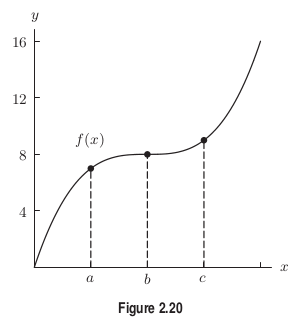
\includegraphics[height=3.5in]{Problem-CT-2-4-9}
\end{center}


\newpage


% 24
%% \item 
%% \label{item:18}
%% Use logarithmic differentiation to find $y'$ if $y = x^{8x}$.
%%  %Compute the drivative of $h(x) = (xe^{2x}-1)^3$.
%% \vskip5cm
%% \hfill {\bf Answer:} $y' = $ \phantom{XXXXXXXXXXXXXXXXXX}\\
%% \phantom{XX} ~ \hfill  \underline{\phantom{XXXXXXXXXXXXXXXXXX}}

%% Evaluate the following limit:
%% \[
%% \lim_{x\rightarrow 1} \frac{x^7 - 1}{x^6-1}
%% \]
%%  %Compute the drivative of $h(x) = (xe^{2x}-1)^3$.
%% \vskip3cm
%% \hfill {\bf Answer:}  \phantom{XXXXXXXXXXXXXXXXXX}\\
%% \phantom{XX} ~ \hfill  \underline{\phantom{XXXXXXXXXXXXXXXXXX}}



%% \item The radius of a sphere is increasing at a rate of 3 mm/s. How fast is the volume
%% increasing when the radius 10 mm? [{\it Hints:}   The volume of a sphere is
%%   $\frac{4}{3}\pi r^3$. The answer is an integer multiple of $\pi$. That is, you
%%   should simplify  your answer so that it is some whole number times $\pi$.]
%% \vskip1in
%% \item Each side of a square is increasing at a rate of 2 cm/s. At what rate is
%%   the area of the square increasing when the area of the square is 49
%%   $\mathrm{cm}^2$? 
%% \vskip5.5cm
%% \hfill {\bf Answer:} $A'= $ \phantom{XXXXXXXXXXX}$\mathrm{cm}^2/\mathrm{s}$ \\
%% \phantom{XX} ~ \hfill  \underline{\phantom{XXXXXXXXXXXXXXX}}

%% \begin{enumerate}[(a)]
%% \item $3(xe^{2x}-1)^2(e^{2x} +2xe^{2x})$
%% \item $3(xe^{2x}-1)^2(xe^{2x} +2x^2e^{2x})$
%% \item $(xe^{2x}-1)^3(e^{2x} +2xe^{2x})$
%% \item $3(e^{2x}+2xe^{2x})^22xe^{2x}$
%% \item none of the above
%% \end{enumerate}
\item A boat is pulled toward a dock by means of a rope wound on a drum that is
  located 3 meters above the bow of the boat. If the rope is being pulled in at the
  rate of 8 meters per minute, how fast is the boat approaching the dock at the time
  $t_1$ when it is 4 meters from the dock?
\begin{center}
  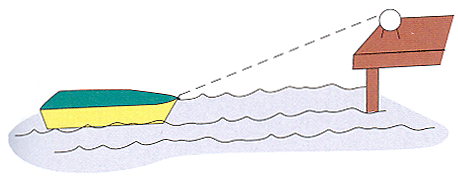
\includegraphics[height=2in]{Prob-3-6-58}
\end{center}
\noindent ({\it Hints:} 
define functions $d(t)$ and $h(t)$ representing distances
at time $t$ from the boat to the dock and drum, respectively; 
relate $d(t)$ and $h(t)$ using the Pythagorean Theorem; differentiate
implicitly, then plug in the given data and solve for $d'(t_1)$.)

\vfill

\hfill {\bf Answer:} $d'(t_1)= $ \phantom{XXXXXXXXXXXXX}meters/min \\
\phantom{XX} ~ \hfill  \underline{\phantom{XXXXXXXXXXXXXXXXXXXXX}}
\newpage

%% \item 
%% Consider the function $f(x) =  1 + (x - 1)^2$ restricted to the closed interval 
%% $[-3, 4]$.  
%% \begin{enumerate}[(a)]
%% \item 
%% Graph this function over the given interval, $-3 \leq x \leq 4$.
%% \begin{center}
%% %\includegraphics[height=6in,width=6.25in]{400px-Graph-paper}
%% \includegraphics[height=4in]{400px-Graph-paper}
%%   \end{center}

%% \item Does $f(x)$ have an 
%% absolute maximum on the interval $-3 \leq x \leq 4$?\\[4pt]
%%   If yes, what is this value?

%% \vskip3cm

%% \item Does $f(x)$ have an 
%% absolute minimum on the interval $-3 \leq x \leq 4$?\\[4pt]
%%   If yes, what is this value?

%% \end{enumerate}

%% \item 
%% Find the absolute maximum and absolute minimum values of 
%% $f(x) = x3 - 6x2 + 9x + 6$ on the interval $[-1, 5]$.

%% \item If $f(3) = 10$ and $f'(x) \geq 3$ for $3 \leq x \leq 7$, how small can
%%   $f(7)$  possibly be?

%% \item
%% \begin{minipage}[t]{0.35\textwidth}
%% According to a recent study, it cost Def Jam Records \$1,078,000
%% to produce Rihanna's single ``Man Down.''\\[1cm]
%% %  (\$78,000 for musicians and
%% % songwriters, and \$1,000,000 for marketing and promotion of the single).
%% Suppose the revenue generated from downloads of the song, as a function of price $p$, is given by
%% \[
%% R(p) = \frac{12000000p}{p^2+9}.
%% \]
%% \end{minipage}
%% %second column
%% \begin{minipage}[t]{0.65\textwidth}
%% \vskip-4mm
%%   \begin{center}
%%   \includegraphics[height=3.5in]{RihannaCost}
%%   \end{center}
%% \end{minipage}

%% \bigskip

%% What price should Def Jam charge for each download in order to
%%   maximize revenue? (Show your work and explain your reasoning.)
%% \ifthenelse{\boolean{answers}}{\\[4pt]Answer: (b) \$1.}{}
%% %% \item Find the absolute maximum and absolute minimum values of
%% %% $f(x) = x^3 - 3x + 1$ on the interval $[0,3]$.


%% \newpage
\newcommand{\qedsymbol}{\underline{\phantom{XX}} }
\item Consider the function $f(x) = 170 + 8x^3 + x^4$.  Find the intervals of
  increase/decrease, local extrema, and the intervals where $f$ is concave
  up/down. %% , and the inflection points of $g$.
  Indicate your answers by placing
  check marks in the appropriate places below.\\[4pt]
\emph{Show your work in the space provided.} (no work $\Rightarrow$ no credit)

\vskip12cm

  \begin{enumerate}[(a)]

\item 
On what interval(s) is $f(x)$ increasing? (Select all that apply.)\\[4pt]
\qedsymbol $(-\infty, -6)$ 
\hfill
\qedsymbol $(-\infty, -4)$
\hfill
\qedsymbol $(-6,0)$
\hfill
\qedsymbol $(0,\infty)$
\hfill
\qedsymbol $(-\infty, 4)$

\vskip5mm

\item 
On what interval(s) is $f(x)$ decreasing? (Select all that apply.)\\[4pt]
\qedsymbol $(-\infty, -6)$ 
\hfill
\qedsymbol $(-\infty, -4)$
\hfill
\qedsymbol $(-6,0)$
\hfill
\qedsymbol $(0,\infty)$
\hfill
\qedsymbol $(-\infty, 4)$

%% \qedsymbol $(-\infty, -6)$
%% \hfill
%% \qedsymbol $(-6, 6)$
%% \hfill
%% \qedsymbol $(-\infty, -4)$
%% \hfill
%% \qedsymbol $(-6,\infty)$
%% \hfill
%% \qedsymbol $(0,\infty)$

\vskip5mm

\item For what $x$ value(s) does $f(x)$ have a local maximum? (Select all that apply.)\\[4pt]
\qedsymbol $-6$
\hfill
\qedsymbol $-4$
\hfill
\qedsymbol $0$
\hfill
\qedsymbol $6$
\hfill
\qedsymbol none of these

\vskip5mm

\item For what $x$ value(s) does $f(x)$ have a local minimum? (Select all that apply.)\\[4pt]
\qedsymbol $-6$
\hfill
\qedsymbol $-4$
\hfill
\qedsymbol $0$
\hfill
\qedsymbol $6$
\hfill
\qedsymbol none of these

\vskip5mm

\item On what interval(s) is the graph of $f(x)$ concave up? (Select all that apply.)\\[4pt]
\qedsymbol $(-\infty, 0)$ 
\hfill
\qedsymbol $(-\infty, -4)$
\hfill
\qedsymbol $(-4,0)$
\hfill
\qedsymbol $(0,\infty)$
\hfill
\qedsymbol $(-6, \infty)$


\vskip5mm

\item On what interval(s) is the graph of $f(x)$ concave down? (Select all that apply.)\\[4pt]
\qedsymbol $(-\infty, -6)$ 
\hfill
\qedsymbol $(-\infty, -4)$
\hfill
\qedsymbol $(-4,0)$
\hfill
\qedsymbol $(0,\infty)$
\hfill
\qedsymbol $(-6, \infty)$


%% \vskip5mm

%% \item The inflection points are:

%% \newpage

%% \item Use this information to sketch the graph of $g(x)$ using the grid below.
%% \end{enumerate}

%% \begin{center}
%% %\includegraphics[height=6in,width=6.25in]{400px-Graph-paper}
%% \includegraphics[height=6in]{400px-Graph-paper}
%%   \end{center}

\end{enumerate}
  \end{enumerate}
\newpage

\begin{center}
  - scratch -
\end{center}



\end{document}
%%%%%%%%%%%%%%%%%%%%%%%%%%%%%%%%%%%%%%%%%%%%%%%%%%%%%%%%%%
%%%%%%%%%%%%%%%%%%%%%%%%%%%%%%%%%%%%%%%%%%%%%%%%%%%%%%%%%%
%%%%%%%%%%%%%%%%%%%%%%%%%%%%%%%%%%%%%%%%%%%%%%%%%%%%%%%%%%

\newpage

{\bf Short answer section.}

\item
\label{item:1}
\begin{enumerate}[i.]
Write down the definition of the derivative of $f(x)$. 
(Use the definition involving a limit.)

\bigskip

\bigskip

\bigskip


$f'(x) = $
\bigskip

\bigskip

\bigskip

\bigskip

\end{enumerate}

\medskip

\item 
\emph{Velocity} is a function $v(t)$ that measures the rate of change of
position.
\emph{Acceleration} is a function $a(t)$ that measures the rate of change of
velocity. 
Suppose your position at time $t$ is given by the function $p(t) = 3t^2 +t$. 
\begin{enumerate}[{\it i.}]
\item 
Use the definition of derivative that involves a limit
(the one you gave in Problem~\ref{item:1}) to compute your velocity
at time $t=2$. (Show your work!  Use a limit for full credit.) 
\\\\
{\it Your work:}

\vskip6cm

\hfill {\bf Answer:} $v(2) = $  \underline{\phantom{XXXXXXX}}

\vskip2cm

\item If your velocity at time $t=2$ is constant, what is your
  acceleration at $t=2$?

\vskip2cm

\hfill {\bf Answer:} $a(2) = $  \underline{\phantom{XXXXXXX}}

\end{enumerate}

